\chapter{ESC characterization}
This section will introduce the different experiments realized to characterize the ESC input-output behavior. For all of them, the real-time data was recorded using the "logger" provided in PX4 that allows to store topics in the SD card connected to the circuit board. The topics logged were:
\begin{itemize}
	\item "actuator\_controls\_0", to see the control signal send to the ESCs.
	\item "esc\_status", to check the rotor speed RPM.
	\item "adc\_report" to read the current sensor analog signal.
\end{itemize}

\section{Sensing Evaluation}
The purpose of this experiment is to determine the quality of the measurements that the ESC provides. The focus is on rotor speed measurements and current sensing. For both experiments in this section (rpm and current sensor validation), a staircase throttle signal was sent and the steady state values were used. Figure \ref{fig:sensing_validation} shows typical experiment data for this section. All experiments were performed with the same set of propellers described in the previous section.

\begin{figure} 
    \centering
    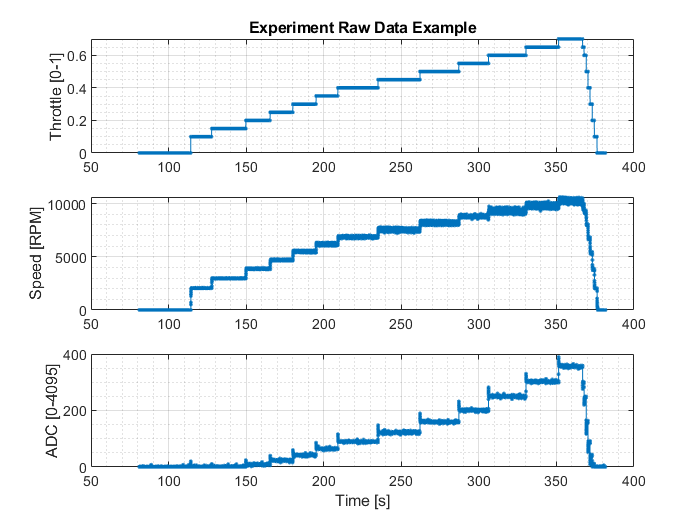
\includegraphics[width=0.6\textwidth]{images/experiment_sample_data.png}
    \caption{Sensing Validation Experiment Example}
    \label{fig:sensing_validation}
\end{figure}

\subsection{ESC RPM feedback}
Experiment in the figure above was repeated 7 times to obtain more data. Here, the rotor speed was measured using the manual tachometer and comparing it to the RPM measurements coming from the ESC. Figure \ref{fig:rpm_validation} shows this relationship. There is very high accuracy and a strong linear behavior. For instance, the fitted curve is characterized as in \ref{eq:rpm_validation}. Notice the high $R^2$ value and slope of $1$. Accordingly, the average relative error is $0.6366\%$

\begin{equation}
  RPM_{actual} = 1.0064RPM_{ESC}-1.523 \quad with \quad R^2=0.999\, .
    \label{eq:rpm_validation}
\end{equation}

\begin{figure} 
    \centering
    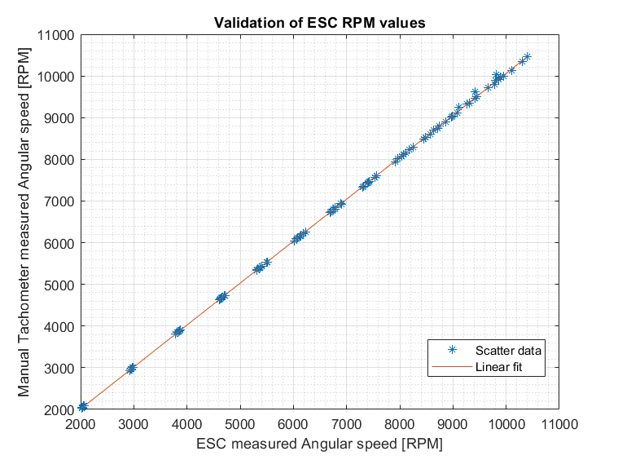
\includegraphics[width=0.6\textwidth]{images/rpm_validation.png}
    \caption{Validation of RPM measurements}
    \label{fig:rpm_validation}
\end{figure}

Therefore, the RPM measurement is accurate enough to be used for feedback control purposes. The accuracy is expected to be high because the ESC needs to have angular estimates of the rotor positioning in order to run and rotor speed is internally calculated by counting revolutions in a fixed period.

\subsection{ESC current sensing}
Another important sensor, to calculate power consumption and in the future help estimate time of flight more accurately is the current sensor. 
\newline

There are two trends to send this information: digitally via an element in the Dshot packet or analogically. In both cases, the the measurement is done via a shunt resistor and the voltage across it will be measured with an ADC. In the digital case, the ADC is located in the ESC and therefore the current estimation is calibrated with the nominal shunt-resistor value. In the analog case, the ADC needs to be in the flight controller. These shunt resistors are usually of $5\%$ tolerance, hence the current measurements need to be calibrated accordingly. This is impossible in the digital case if the firmware is closed-source.\\

As the measurement is shunt resistor based, it is expected that the relationship is highly linear. This is confirmed in Figure \ref{fig:current_validation} that was used to calibrate the current sensor measurement. 
\begin{figure} 
    \centering
    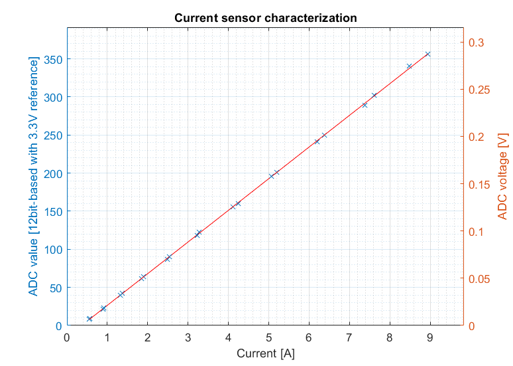
\includegraphics[width=0.6\textwidth]{images/current_validation.png}
    \caption{Validation of current measurements}
    \label{fig:current_validation}
\end{figure}

\section{Motor-drive dynamics}

\subsection{RPM-Voltage-Throttle relation}
As shown in previous literature, the rotor speed also varies with respect to battery voltage. Therefore, an experiment similar to the one described in Figure \ref{fig:sensing_validation} was set up for different battery voltages that were varied using a power supply. After analyzing the data, one can see that even though the voltage does not change the output as dramatically as throttle does, the variation is significant for instance it appears linear when looking at the cross-section. It is also coherent with theory as higher voltages generate linearly related higher currents and therefore higher induced magnetic field. In the end, this allows for higher torques and steady state rotor speed.\\

Furthermore, a significant non-linearity can be observed in the dependence from throttle. The reason for this is the way the ESC approximates driving voltages (switching transistors) because it introduces high frequency current components that can pass through parasitic capacitances and the MOSFETs body diodes in the circuit. Therefore, augmenting from the linear throttle dependency model explained in \cite{Moutinho2015}, the quadratic model in Equation \ref{eq:rmp_V_throt_quad} is introduced to account for non-linearities. The parameters were found using Non-linear least squares optimization method given the test data.
\begin{equation}
\begin{split}
 \omega &= (at^2 +bt+c)V\, .\\
 a&=-7.038\times 10^{-5}\\
 b&=0.4155\\
 c&=3.168
\end{split} 
\label{eq:rmp_V_throt_quad}   
\end{equation}

Figure \ref{fig:rpm_fit} shows the data points as black dots and the surface represents the model proposed above. The fit provided a good approximation with $R^2=0.996$ and on average $1.5\%$ error in rotor speed obtained.

\begin{figure} 
    \centering
    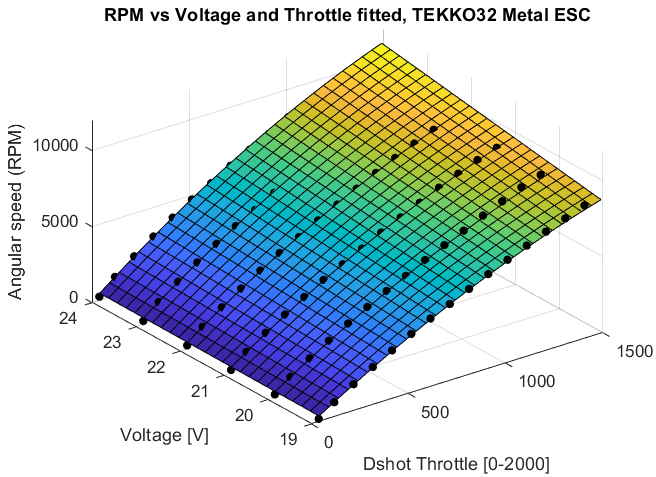
\includegraphics[width=0.65\textwidth]{images/surf_rpm_model.png}
    \caption{RPM dependence on throttle and voltage}
    \label{fig:rpm_fit}
\end{figure}



\subsection{ESC to ESC discrepancies}
Given the complexity of the OMAV and that the current control assumes equal throttle to RPM mapping for all ESCs, this investigation also assessed the  variability in rotor speed depending on the hardware used. To do so, different ESC-motor combinations were subject to staircase-like signals as in the previous experiments. Two factors were considered into this analysis: motors and ESCs. Indeed, significant variations for different motors and ESCs combinations were found as it is summarized in Figure \ref{fig:esc_dis_all_rpm} and \ref{fig:esc_dis_all_thrust}.\\

\begin{figure}[!tbp]
  \centering
  \makebox[\textwidth]{
  \subfloat[RPM]{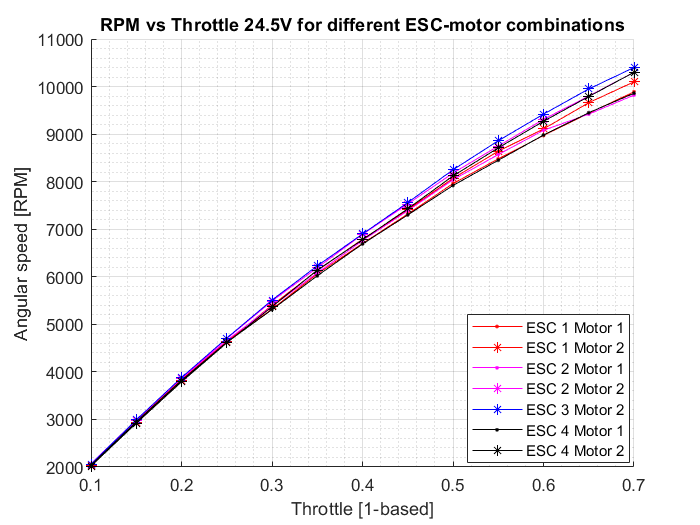
\includegraphics[width=0.65\textwidth]{images/esc_dis_all_rpm.png}\label{fig:esc_dis_all_rpm}}
  \hfill
  \subfloat[Thrust]{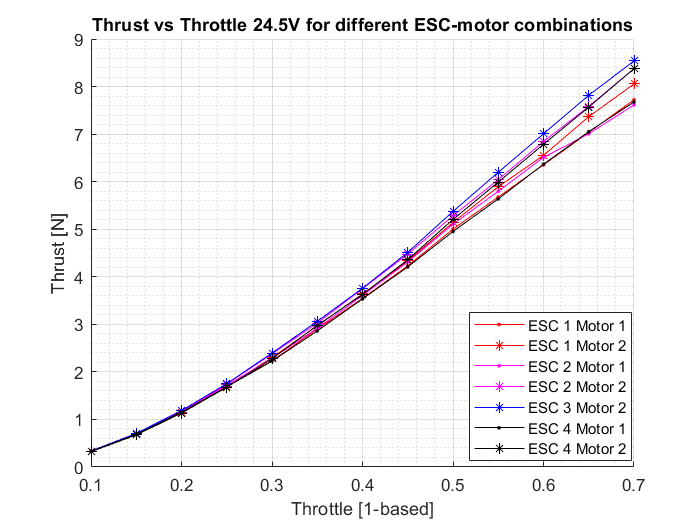
\includegraphics[width=0.65\textwidth]{images/esc_dis_all_thrust.png}\label{fig:esc_dis_all_thrust}}
  }
  \caption{Discrepancies for different ESC-motor responses
  \label{fig:esc_discrepancies_overall}}
\end{figure}

From Figure \ref{fig:esc_discrepancies_overall}, we can see that variations between same-model parts can cause discrepancies of $5\%$ in rotor speed and $10\%$ in thrust generated. Therefore, calibration is key. Additionally, Figure \ref{fig:esc_mot_stats} shows the representation of these measurements as Gaussian random variables with the the mean and double standard deviation range (for $95\%$ confidence interval). Note that the standard deviation increases with throttle too. With this model, the variability range for rotor speed was was up to $1.5N$ and $960RPM$ at high throttle. Therefore, system identification is recommended to be in a motor-ESC pair basis. Two of the factors that could cause this variation were isolated and tested separately, to see individual contributions to uncertainty. That is, testing with different motors for a fixed ESC and vice versa. 



\begin{figure}[!tbp]
  \centering
  \makebox[\textwidth]{
  \subfloat{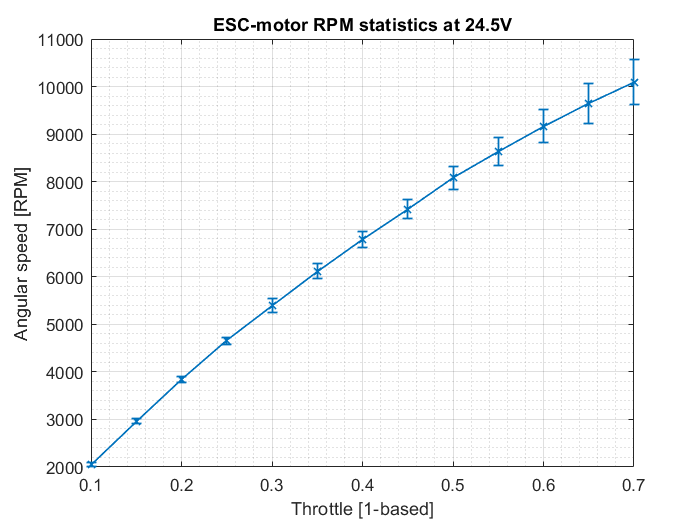
\includegraphics[width=0.6\textwidth]{images/esc_mot_stats_rpm.png}}
  \hfill
  \subfloat{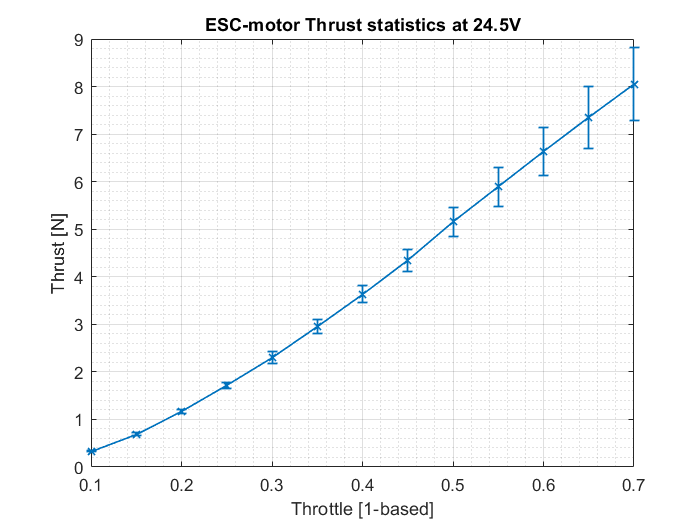
\includegraphics[width=0.6\textwidth]{images/esc_mot_stats_thrust.png}}
  }
  \caption{ESC-motor combination characterization showing mean and 2 standard deviation range}
  \label{fig:esc_mot_stats}
\end{figure}

\subsubsection{Motor differences}
For this analysis, the experiments with the same ESC but different motor were analyzed. A typical curve analyzed in this section is shown in Figure \ref{fig:mot_discr}. Again, the difference between the response with two motors increases with throttle, reaching $440RPM$ in speed and $0.7N$ in thrust at 0.7 throttle. \\

Higher rotor speed values accentuate this difference more that lower ones. This suggests that a viscous friction element acting differently since the same propeller is used. The reason to suggest viscous friction are the ball bearings. In fact, \cite{Armstrong-H1994} studied friction for robotic machines, where bearings are explained to have a representative viscous friction component.\\

Another element contributing to higher viscous friction would be slight miss-alignments when manufacturing the motors. That is, axis-bearing misalignments that would result bearing load increase , which in turn rises friction torque.

\begin{figure}[!tbp]
  \centering
  \makebox[\textwidth]{
  \subfloat{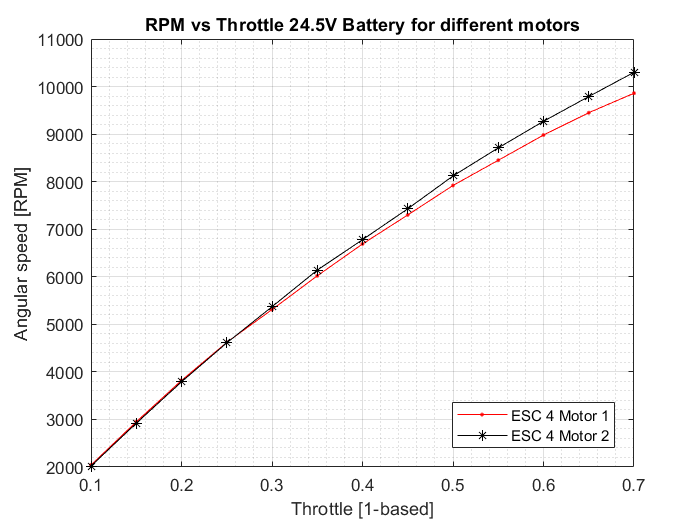
\includegraphics[width=0.6\textwidth]{images/motor_discrepancy_rpm.png}}
  \hfill
  \subfloat{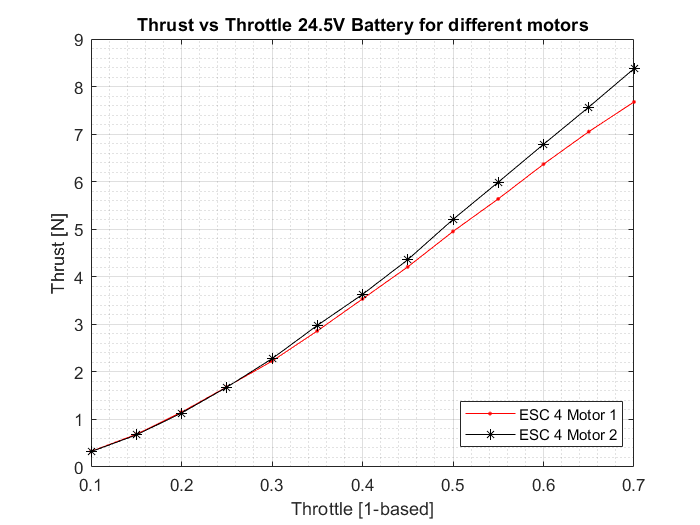
\includegraphics[width=0.6\textwidth]{images/motor_discrepancy_thrust.png}}
  }
  \caption{Comparison of different motors response}
  \label{fig:mot_discr}
\end{figure}


\subsubsection{ESC differences}
To analyze this, the 4 individual ESCs of a TEKKO board were compared using the same motor, taking the corresponding subset from the data in Figure \ref{fig:esc_discrepancies_overall}. The data statistics is compiled in Figure \ref{fig:esc_esc_stats} by including taking the mean and 2 standard deviation range for $95\%$ confidence interval. Even though the individual ESCs belong to the same model, significant variation can be seen. For instance, it shows the $95\%$ intervals can be as high as $503RPM$ in rotor speed and $0.81N$ in thrust at 0.7 throttle. In 
absolute terms, the largest discrepancy was  $300RPM$ in speed and $0.49N$ in thrust at 0.7 throttle. It is also noticeable that these disparities increase with throttle. 


\begin{figure}[!tbp]
  \centering
  \makebox[\textwidth]{
  \subfloat{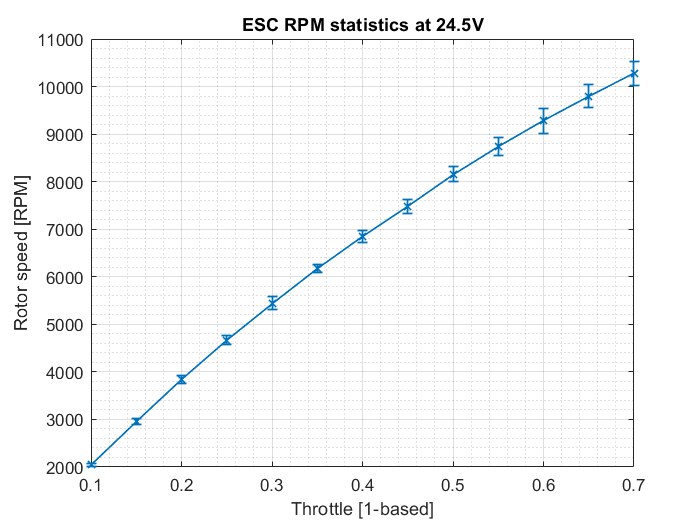
\includegraphics[width=0.6\textwidth]{images/esc_esc_rpm_stats.png}}
  \hfill
  \subfloat{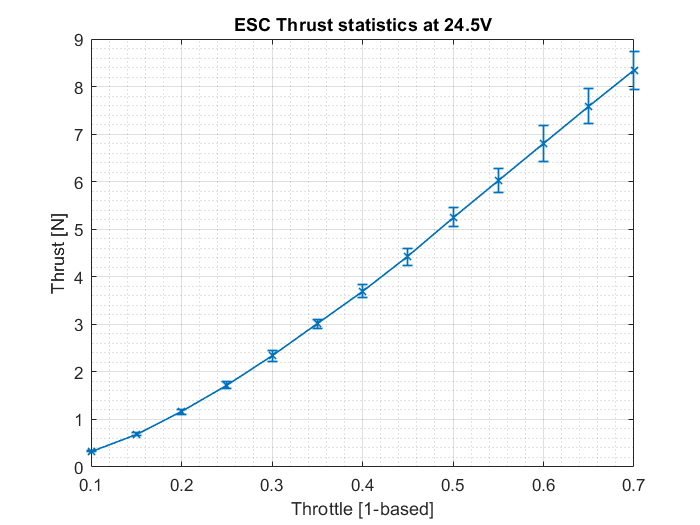
\includegraphics[width=0.6\textwidth]{images/esc_esc_thrust_stats.png}}
  }
  \caption{Different ESCs responses statistics}
  \label{fig:esc_esc_stats}
\end{figure}

The different behavior of same model ESCs can be explained mainly by the tolerances and imperfection of it's components. For instance, a big contributor is the shunt resistor used to measure current. These usually have $5\%$ tolerance (which is also wise to calibrate the current measurement). To analyze the impact this has, the MOSFET to rotor windings connection is simplified to DC analysis as it is the main components that drives the motor. Therefore, the simplified circuit for each "on" part of the driving looks is in Figure \ref{fig:shunt_circuit}, given the connection of shunt resistors shown in Figure \ref{fig:esc_diag}.

\begin{figure}
  \centering
  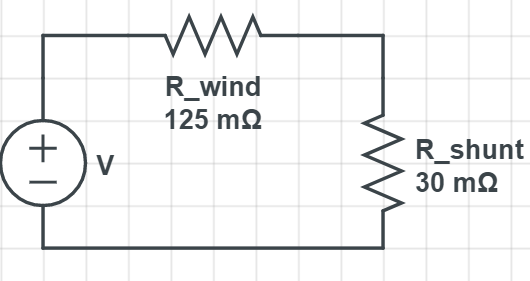
\includegraphics[width=0.4\textwidth]{images/shunt_circuit.png}
  \caption{Shunt circuit simplification}
  \label{fig:shunt_circuit}
\end{figure}

With this simplified system, one can calculate the voltage across the motor active windings and then obtain the difference for maximum variation in shunt resistor, using Equation \ref{eq:winding_volt_div}. The winding resistance was taken as $R_{wind}=125m\Omega$ from the motor data-sheet \cite{KDE-Direct2020} and the shunt resistor as $R_{shunt}=30m\Omega$ from the ESC board. With this values, the maximum discrepancy between equivalent DC component voltage applied is $2\%$ of the source voltage.

\begin{equation}
\begin{split}
 V_{wind-dif} &= abs\left(\frac{R_{wind}}{R_{wind}+R_{shunt}}-\frac{R_{wind}}{R_{wind}+R_{shunt}\pm tol}\right)V 
\end{split} 
\label{eq:winding_volt_div}   
\end{equation}

Another big contributor to this discrepancies due to ESCs non-uniformity is the switching loss. This corresponds to the power losses caused by the high frequency current peaks generated by the switching but also by the time during turning on-off transients, causing interferences between waveform sections and current flows in places where none is planned. Hence, these losses come from three different physical roots \cite{Keskar,Kahrimanovic2016}:

\begin{itemize}
	\item Conduction loss. This refers to the power loss within each MOSFET, when they are turned on. and it is given by: $P_{cond}=V_{rms}^2/R_{DSon}$ where the drain to source resistor $R_{DSon}$ is less than $1.2m\Omega$ (typically $0.9m\Omega$) obtained from the MOSFETs data-sheet \cite{Infineon2016}
	\item Switching loss. This corresponds to the time it takes to transition from low to high states in each MOSFET. It is calculated for rising and falling edges as  $P_{switch}=0.5V\times I\times t_R\times f_{sw}$. Where $t_R$ is the switching time and $f_{sw}$ the modulation frequency.
	\item Diode loss happens during the dead-time between commutation transitions (i.e. all MOSFETs are off in this time). When there is a deadtime, the instantatnous current must flow through some component. For instance, it finds a path through the body diode of the lower MOSFETs (See Fig. \ref{fig:bldcm}). The body diode forward voltage is given with a high uncertainty in the data-sheet as maximum of $1.2V$ \cite{Infineon2016} but without a minimum threshold. Therefore, this is expected to give significant variability between ESCs of the same model.

\end{itemize}


\subsection{Transient response and active break}
Another important characteristic for control, specially if cascade controllers are used (usually the case in UAVs), is the speed of the system when reacting to a command. This experiment aims to determine this characteristic by commanding rising and falling steps of different amplitudes. This was performed for the case with active and inactive brake \footnote{This feature is activated in the ESC firmware, BLHeli\_32. Instructions of how to change it are found in Appendix \ref{sec:firm_blheli}}. A typical signal and it's response used to measure both rise and fall transitions is shown in Figure \ref{fig:time_const_signals}. Note that the response shows first order characteristics as no overshoot is seen, which was the case for all step sizes.\\

\begin{figure}
  \centering
  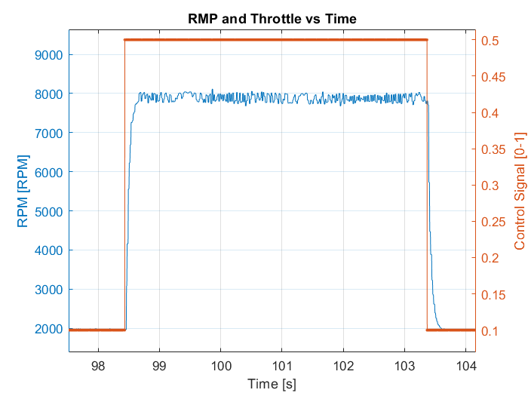
\includegraphics[width=0.6\textwidth]{images/time_constant_signals.png}
  \caption{Signal used to characterize speed of response}
  \label{fig:time_const_signals}
\end{figure}

The time constant of these signals was computed for each step size by measuring the time take to reach $63\%$ of the steady state point. Figure \ref{fig:time_const_plot} summarizes these results.

\begin{figure}
  \centering
  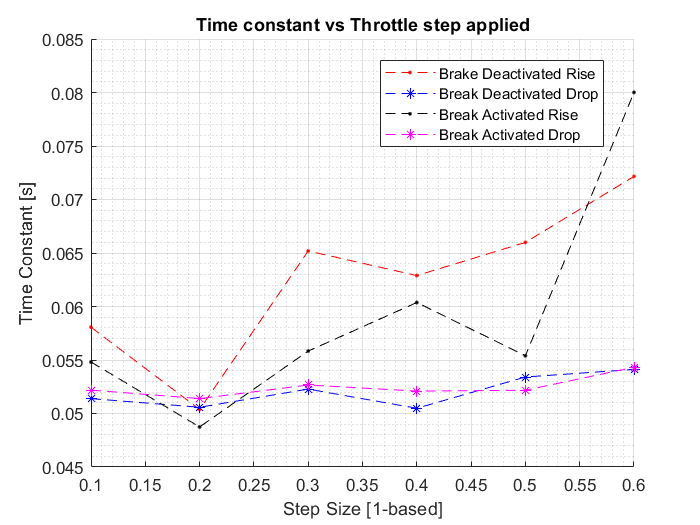
\includegraphics[width=0.6\textwidth]{images/time_const_plot.png}
  \caption{Speed response Rise time for different active break and edge direction settings}
  \label{fig:time_const_plot}
\end{figure}

The first fact to notice is that there is no distinctive trend that allows to discern active brake effects on speed of the response. However, we see a lower time constant for the falling edge case, averaging at $52,5ms$ for all step sizes which is not the case for the rising edges whose rise time changes from $49ms$ to $80ms$ with an overall increasing trend with rising step size. Consequently, the only possible explanation for the falling edge time constant being lower than the rising edge is that the active brake is always active in this particular ESC. Therefore, this implies that the response is non-linear and therefore is very difficult to model in frequency domain.\\

From the same data collected, the maximum acceleration in rising and falling steps was calculated, encountering a maximum $9616\tfrac{rad}{s^2}$ rising acceleration and $8317\tfrac{rad}{^s2}$ falling acceleration.


\subsection{Coaxial rotor interference}
A special characteristic of the OMAV in question, is the coaxial position of propellers. The interference was analyzed by performing staircase signals as in Fig. \ref{fig:sensing_validation} for both rotors in the Fig. \ref{fig:exp_setup} setup simultaneously. The steady state values were used for analysis.\\

Figure \ref{fig:mot_interference} compares the response of bottom and top propellers when run individually opposed to when run together. It can be clearly seen that when both propellers are run together, the Bottom motor increases in speed. For instance, the error in comparison to the individual rises up to $5.2\%$ or $510RPM$ at 0.7 throttle. This variation also increases with increasing throttle. Regarding the top propeller, it did not show significant change when run together, for instance only $1\%$ error. \\

The speed increase in the lower propeller is explained by two facts: no feedback control is performed; and the top propeller induces a downward flow that pushes the bottom blades in the same direction of motion. Since the equilibrium rotor speed is dependent on the load it gets and the flow provided by the top motor would generate a favorable torque in the bottom propeller, the equilibrium rotor speed at the lower side will be higher. \\

\begin{figure}
  \centering
  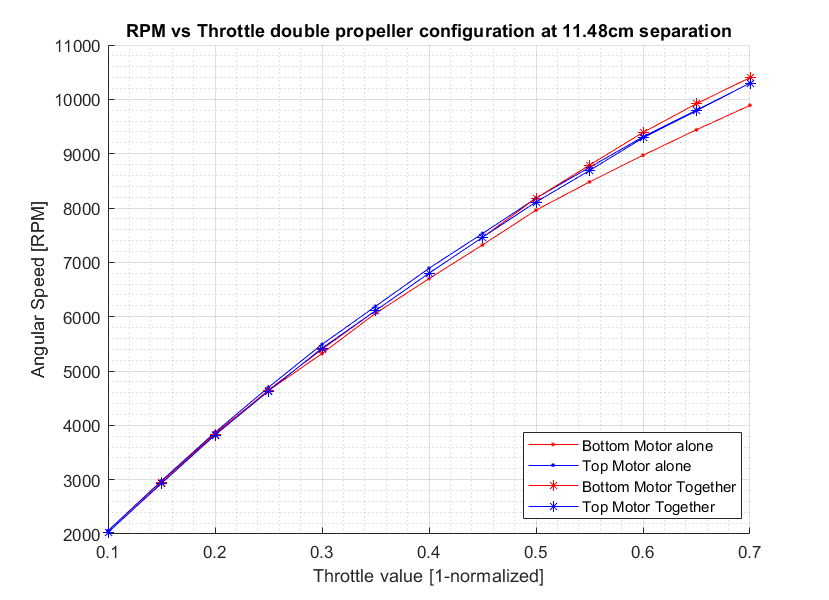
\includegraphics[width=0.9\textwidth]{images/mot_interference.png}
  \caption{Interference between coaxially aligned motors}
  \label{fig:mot_interference}
\end{figure}

To summarize, this discrepancy is caused by the different air inlet speeds in the top and bottom propeller that cause different aerodynamic torques in each propeller.


\section{Frequency Modulation and Efficiency}

The last element analyzed in during the project was the effect of activating Sine Modulation mode and using different modulation frequencies for the motor driving signals \footnote{Setup within BlHeli\_32 as shown in Appendix \ref{sec:firm_blheli}}. Hence, a staircase signal as in the previous sections was used for each combination of modulations ($16kHz$, $24kHz$ and $48kHz$) with and without sine mode. in BlHeli\_32 sine mode is an approximation to FOC. The speed curves did not show significant reference. However, the efficiency does change. As shown in Figure \ref{fig:efficiency_characterization}, higher modulation frequencies show less current consumption to achieve fixed rotor speeds. This implies that more thrust would be obtained for less electrical power, hence more efficient.\\

Higher efficiency comes from a better driving signal, explained more thoroughly in Section \ref{sec:bldc_driving_methods}.

\begin{figure}
  \centering
  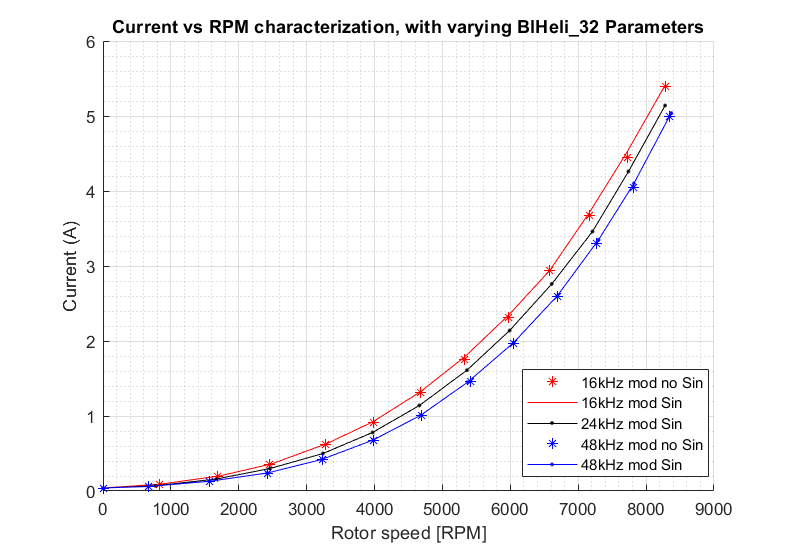
\includegraphics[width=0.9\textwidth]{images/efficiency_characterization.png}
  \caption{Current consumed for different modulation parameters}
  \label{fig:efficiency_characterization}
\end{figure}
